\documentclass{article}   
\usepackage[left=1.5cm,right=1.5cm,top=2.3cm,bottom=2.3cm]{geometry}		
\usepackage[utf8]{inputenc} 										
%\usepackage[french]{babel}
\usepackage{fancyhdr}										
\usepackage{hyperref}										
\usepackage{booktabs,multirow,hhline}							
\usepackage{graphicx}									
\usepackage{wrapfig,caption}
\usepackage{subcaption}
\usepackage[compact]{titlesec}
\titlespacing{\section}{0pt}{2ex}{1ex}
\titlespacing{\subsection}{0pt}{1ex}{0ex}
\titlespacing{\subsubsection}{0pt}{0.5ex}{0ex}
\usepackage{color}												
\usepackage[dvipsnames]{xcolor}								
\usepackage{amsmath,amssymb,amsthm,nicefrac}
\usepackage{mathrsfs}										
\usepackage{wasysym,marvosym}
\usepackage{mathtools}
\usepackage{verbatim}										
\usepackage{minted}										
\usepackage{lipsum}
\usepackage{tikz}
\usepackage[american]{circuitikz}
\usepackage{siunitx}
\usepackage{physics}
\usepackage{float}
%\usepackage{biblatex}
\usepackage{movie15}
\usepackage{multicol}
%\usepackage[backend=biber, style=numeric]{biblatex}

%\newenvironment{Figure}
%{\par\medskip\noindent\minipage{\linewidth}}
  %{\endminipage\par\medskip}

\parindent=0pt									
\parskip=6pt									

\fancyheadoffset{0 cm}	

%---------------
\begin{document}

\begin{center}

    {\Large \textbf{Quantitative assessment of spatial smoothing-induced correlations}}\\
    
    \vspace{10 pt}
    Olivier Ribordy$^{1}$ \\
    \vspace{5 pt}
    
    $^1$\textit{Département de physique, de génie physique et d'optique, Université Laval, Québec (Québec), Canada}
    

\end{center}

\vspace{10 pt}

\begin{multicols}{2}

\section*{Introduction}



\section*{Results}


\subsection*{Correlations emerging from spatial smoothing of gaussian noise signals}

We investigate the artifical introduction of correlations by the use of spatial smoothing on node activity in graphs embedded in a metric space. In the following, correlations will be taken as the Pearson correlation coefficient,  which, for a sample of variables $x$ and $y$ of size $n$, is given by
\begin{align*}
    r_{xy} = \frac{\sum_{i=1}^n(x_i-\bar{x})(y_i-\bar{y})}{\sqrt{\sum ^n _{i=1}(x_i - \bar{x})^2} \sqrt{\sum ^n _{i=1}(y_i - \bar{y})^2}},
\end{align*}
where $\bar{x}$ and $\bar{y}$ are the average values of $x$ and $y$. Since we are interested in the expected value of this coefficient for random signals, we will instead proceed with our calculations using the following coefficient:
\begin{align}
    c_{ij} &= \frac{\expval{f_if_j}-\expval{f_i}\expval{f_j}}{\sigma_{f_i}\sigma_{f_j}},
    \label{eq:exp_coefficient}
\end{align}
where $f_i$ would be the random variable corresponding to the activity of node $i$ on a observed unknown network, for instance. If we treat those signals as independent and with mean $0$, the expected coefficient is simply
\begin{align*}
    c_{ij} &= \frac{\expval{f_i}\expval{f_j}-\expval{f_i}\expval{f_j}}{\sigma_{f_i}\sigma_{f_j}} = 0.
\end{align*}
Now, we introduce spatial smoothing to the signal. This procedure consists of convoluting the signal with a gaussian filter, which yields
\begin{align*}
    \Tilde{f}_i &= \frac{1}{\sqrt{2\pi}\sigma N}\sum_{k=1}^N e^{-\nicefrac{d_{ik}^2}{2\sigma^2}}f_k,
\end{align*}
where $\sigma$ is the standard deviation of the gaussian filter, $N$ is the number of nodes in the network and $d_{ij}$ is the distance between nodes $i$ and $j$. Since all $f_k$ have mean $0$, the smoothed signals $\Tilde{f}_i$ also have mean $0$. The covariance between these smoothed signals is then
\begin{align*}
    \expval{\Tilde{f}_i\Tilde{f}_j} &= \frac{1}{2\pi\sigma^2N^2}\expval{\qty(\sum_{k=1}^N e^{-\nicefrac{d_{ik}^2}{2\sigma^2}}f_k)\qty(\sum_{\ell=1}^N e^{-\nicefrac{d_{j\ell}^2}{2\sigma^2}}f_\ell)}\\
    &= \frac{1}{2\pi\sigma^2N^2}\expval{\sum_{k, \ell =1}^N e^{\nicefrac{-(d_{ik}^2+d_{j\ell}^2)}{2\sigma^2}}f_kf_\ell}\\
    &= \frac{1}{2\pi\sigma^2N^2}\sum_{k, \ell =1}^N e^{\nicefrac{-(d_{ik}^2+d_{j\ell}^2)}{2\sigma^2}}\expval{f_kf_\ell}.
\end{align*}
Since the unsmoothed signals are independent, $\expval{f_kf_\ell} = \expval{f_k^2}\delta_{k\ell} = \delta_{k\ell}$, with $\delta_{k\ell}$ the Kronecker delta. The covariance is therefore
\begin{align*}
    \expval{\Tilde{f}_i\Tilde{f}_j} &= \frac{1}{2\pi\sigma^2N^2}\sum_{k = 1}^N e^{\nicefrac{-(d_{ik}^2+d_{jk}^2)}{2\sigma^2}}.
\end{align*}
For the standard deviations, we have
\begin{align*}
    \sigma^2_{\Tilde{f}_i} &= \expval{\Tilde{f}_i^2}\\
    &= \frac{1}{2\pi\sigma^2N^2}\expval{\qty(\sum_{k=1}^N e^{-\nicefrac{d_{ik}^2}{2\sigma^2}}f_k)\qty(\sum_{\ell=1}^N e^{-\nicefrac{d_{i\ell}^2}{2\sigma^2}}f_\ell)}\\
    &= \frac{1}{2\pi\sigma^2N^2}\expval{\sum_{k, \ell =1}^N e^{-(\nicefrac{d_{ik}^2 + d_{i\ell}^2)}{2\sigma^2}}f_kf_\ell}\\
    &= \frac{1}{2\pi\sigma^2N^2}\sum_{k=1}^N e^{-\nicefrac{d_{ik}^2}{\sigma^2}}.
\end{align*}
The expected correlation between the smoothed signals is then
\begin{align}
    \Tilde{c}_{ij} &= \frac{\sum_{k = 1}^N e^{\nicefrac{-(d_{ik}^2+d_{jk}^2)}{2\sigma^2}}}{\sqrt{\qty(\sum_{k=1}^N e^{-\nicefrac{d_{ik}^2}{\sigma^2}})\qty(\sum_{\ell=1}^N e^{-\nicefrac{d_{j\ell}^2}{\sigma^2}})}} \geq 0.
    \label{eq:artificial_correlation}
\end{align}
The corresponding correlation matrix is presented in figure \ref{fig:correlation matrix}.

\begin{figure}[H]
    \centering    
    \includegraphics[width=0.3\textwidth]{figures/Theoretical correlations.png}
    \caption{Correlation matrix with entries given by equation \ref{eq:artificial_correlation}}
    \label{fig:correlation matrix}
\end{figure}

Simplifying equation \ref{eq:artificial_correlation}, as far as I can tell, requires knowledge of the metric space in which the graph is embedded, of the distribution of the nodes in that metric space and thus of the distribution of the distances between nodes. Even when this information is available, this process is arduous, but we might revisit it later for specific geometries. We can, however, try to isolate the effect of $d_{ij}$ by using the law of cosines in the exponential at the numerator, which yields
\begin{align}
    \Tilde{c}_{ij} &= e^{\nicefrac{-d_{ij}^2}{2\sigma^2}}\frac{\sum_{k = 1}^N e^{\nicefrac{-d_{ik}d_{jk}\cos(\angle ikj)}{\sigma^2}}}{\sqrt{\qty(\sum_{k=1}^N e^{-\nicefrac{d_{ik}^2}{\sigma^2}})\qty(\sum_{\ell=1}^N e^{-\nicefrac{d_{j\ell}^2}{\sigma^2}})}},
    \label{eq:gaussian_correlation}
\end{align}
with $\angle ikj$ denoting the angle between segments $ik$ and $kj$. Although this does leave a dependence on $ij$ in the numerator, equation \ref{eq:gaussian_correlation} still suggests that the smoothed correlations should decrease with distance following a curve proportional to the gaussian filter that was applied.

\subsection*{Artifical correlations introduced to correlated systems}
We now produce a similar analysis, but for systems where the signals are not gaussian noise, and therefore $\expval{f_kf_\ell} \neq \delta_{k\ell}$. In that case,
\begin{align*}
     \expval{\Tilde{f_i}} &= \frac{1}{\sqrt{2\pi}\sigma N}\sum_{k=1}^N e^{-\nicefrac{d_{ik}^2}{2\sigma^2}}\expval{f_k}
\end{align*}
and

\begin{align*}
    \expval{\Tilde{f}_i\Tilde{f}_j} &= \frac{1}{2\pi\sigma^2N^2}\sum_{k, \ell =1}^N e^{\nicefrac{-(d_{ik}^2+d_{j\ell}^2)}{2\sigma^2}}\expval{f_kf_\ell}.
\end{align*}
For the smoothed standard deviations,
\begin{align*}
    \sigma_{\Tilde{f_i}}^2 &= \expval{\Tilde{f_i}^2} - \expval{\Tilde{f_i}}^2.
\end{align*}
Let's calculate each term separately. 
\begin{align*}
     \expval{\Tilde{f_i}}^2 &= \frac{1}{2\pi\sigma^2N^2}\sum_{k=1, \ell=1}^N e^{-\nicefrac{(d_{ik}^2+ d_{i\ell}^2)}{2\sigma^2}}\expval{f_k}\expval{f_\ell}\\
    \expval{\Tilde{f_i}^2} &= \frac{1}{2\pi\sigma^2N^2}\sum_{k=1, \ell=1}^N e^{-\nicefrac{(d_{ik}^2+ d_{i\ell}^2)}{2\sigma^2}}\expval{f_k f_\ell}\\
    \implies \sigma_{\Tilde{f_i}}^2 &= \frac{1}{2\pi\sigma^2N^2}\sum_{k=1, \ell=1}^N e^{-\nicefrac{(d_{ik}^2+ d_{i\ell}^2)}{2\sigma^2}}\qty(\expval{f_k f_\ell} - \expval{f_k}\expval{f_\ell})\\
    &= \frac{1}{2\pi\sigma^2N^2}\sum_{k=1, \ell=1}^N e^{-\nicefrac{(d_{ik}^2+ d_{i\ell}^2)}{2\sigma^2}}c_{k\ell}\sigma_{f_k}\sigma_{f_\ell}
\end{align*}
\end{multicols}
\centering
\rule{0.66\textwidth}{0.4pt}

\raggedright
\vspace{10pt}

Therefore,
\begin{align}
    \Tilde{c}_{ij} &= \frac{\sum_{k, \ell =1}^N e^{\nicefrac{-(d_{ik}^2+d_{j\ell}^2)}{2\sigma^2}}c_{k\ell}\sigma_{f_k}\sigma_{f_\ell}}{\sqrt{\qty(\sum_{k=1, \ell=1}^N e^{-\nicefrac{(d_{ik}^2+ d_{i\ell}^2)}{2\sigma^2}}c_{k\ell}\sigma_{f_k}\sigma_{f_\ell})\qty(\sum_{k=1, \ell=1}^N e^{-\nicefrac{(d_{jk}^2+ d_{j\ell}^2)}{2\sigma^2}}c_{k\ell}\sigma_{f_k}\sigma_{f_\ell})}} \nonumber \\
    &= \frac{e^{\nicefrac{-(d_{ii}^2+d_{jj}^2)}{2\sigma^2}}c_{ij}\sigma_{f_i}\sigma_{f_j} + \sum_{k\neq i, \ell \neq j}^N e^{\nicefrac{-(d_{ik}^2+d_{j\ell}^2)}{2\sigma^2}}c_{k\ell}\sigma_{f_k}\sigma_{f_\ell}}{\sqrt{\qty(\sum_{k=1, \ell=1}^N e^{-\nicefrac{(d_{ik}^2+ d_{i\ell}^2)}{2\sigma^2}}c_{k\ell}\sigma_{f_k}\sigma_{f_\ell})\qty(\sum_{k=1, \ell=1}^N e^{-\nicefrac{(d_{jk}^2+ d_{j\ell}^2)}{2\sigma^2}}c_{k\ell}\sigma_{f_k}\sigma_{f_\ell})}} \nonumber \\
    &= c_{ij}+\frac{\sum_{k\neq i, \ell \neq j}^N e^{\nicefrac{-(d_{ik}^2+d_{j\ell}^2)}{2\sigma^2}}c_{k\ell}\frac{\sigma_{f_k}\sigma_{f_\ell}}{\sigma_{f_i}\sigma_{f_j}}}{\sqrt{\qty(\sum_{k=1, \ell=1}^N e^{-\nicefrac{(d_{ik}^2+ d_{i\ell}^2)}{2\sigma^2}}c_{k\ell}\frac{\sigma_{f_k}\sigma_{f_\ell}}{\sigma_{f_i}\sigma_{f_j}})\qty(\sum_{k=1, \ell=1}^N e^{-\nicefrac{(d_{jk}^2+ d_{j\ell}^2)}{2\sigma^2}}c_{k\ell}\frac{\sigma_{f_k}\sigma_{f_\ell}}{\sigma_{f_i}\sigma_{f_j}})}}.
    \label{eq:additive_correction}
\end{align}
\begin{multicols}{2}
    Some analysis is now needed to evaluate the value of the correction term in equation \ref{eq:additive_correction}. I believe such progress is difficult without knowledge of the geometry or of the unsmoothed correlation values. However, we could reasonably expect the two sums in the denominator to be roughly equal, given that the nodes are uniformly distributed in the space. This should mean that summing a function of the distances between the nodes over all nodes should depend very little on which node is chosen as the "fixed node". If this hypothesis is true,
    \begin{align*}
        \Tilde{c}_{ij} &\approx c_{ij}+\frac{\sum_{k\neq i, \ell \neq j}^N e^{\nicefrac{-(d_{ik}^2+d_{j\ell}^2)}{2\sigma^2}}c_{k\ell}\frac{\sigma_{f_k}\sigma_{f_\ell}}{\sigma_{f_i}\sigma_{f_j}}}{\sum_{k=1, \ell=1}^N e^{-\nicefrac{(d_{ik}^2+ d_{i\ell}^2)}{2\sigma^2}}c_{k\ell}\frac{\sigma_{f_k}\sigma_{f_\ell}}{\sigma_{f_i}\sigma_{f_j}}}.
    \end{align*}
\end{multicols}

%\begin{figure*}[t!]
%    \centering
%    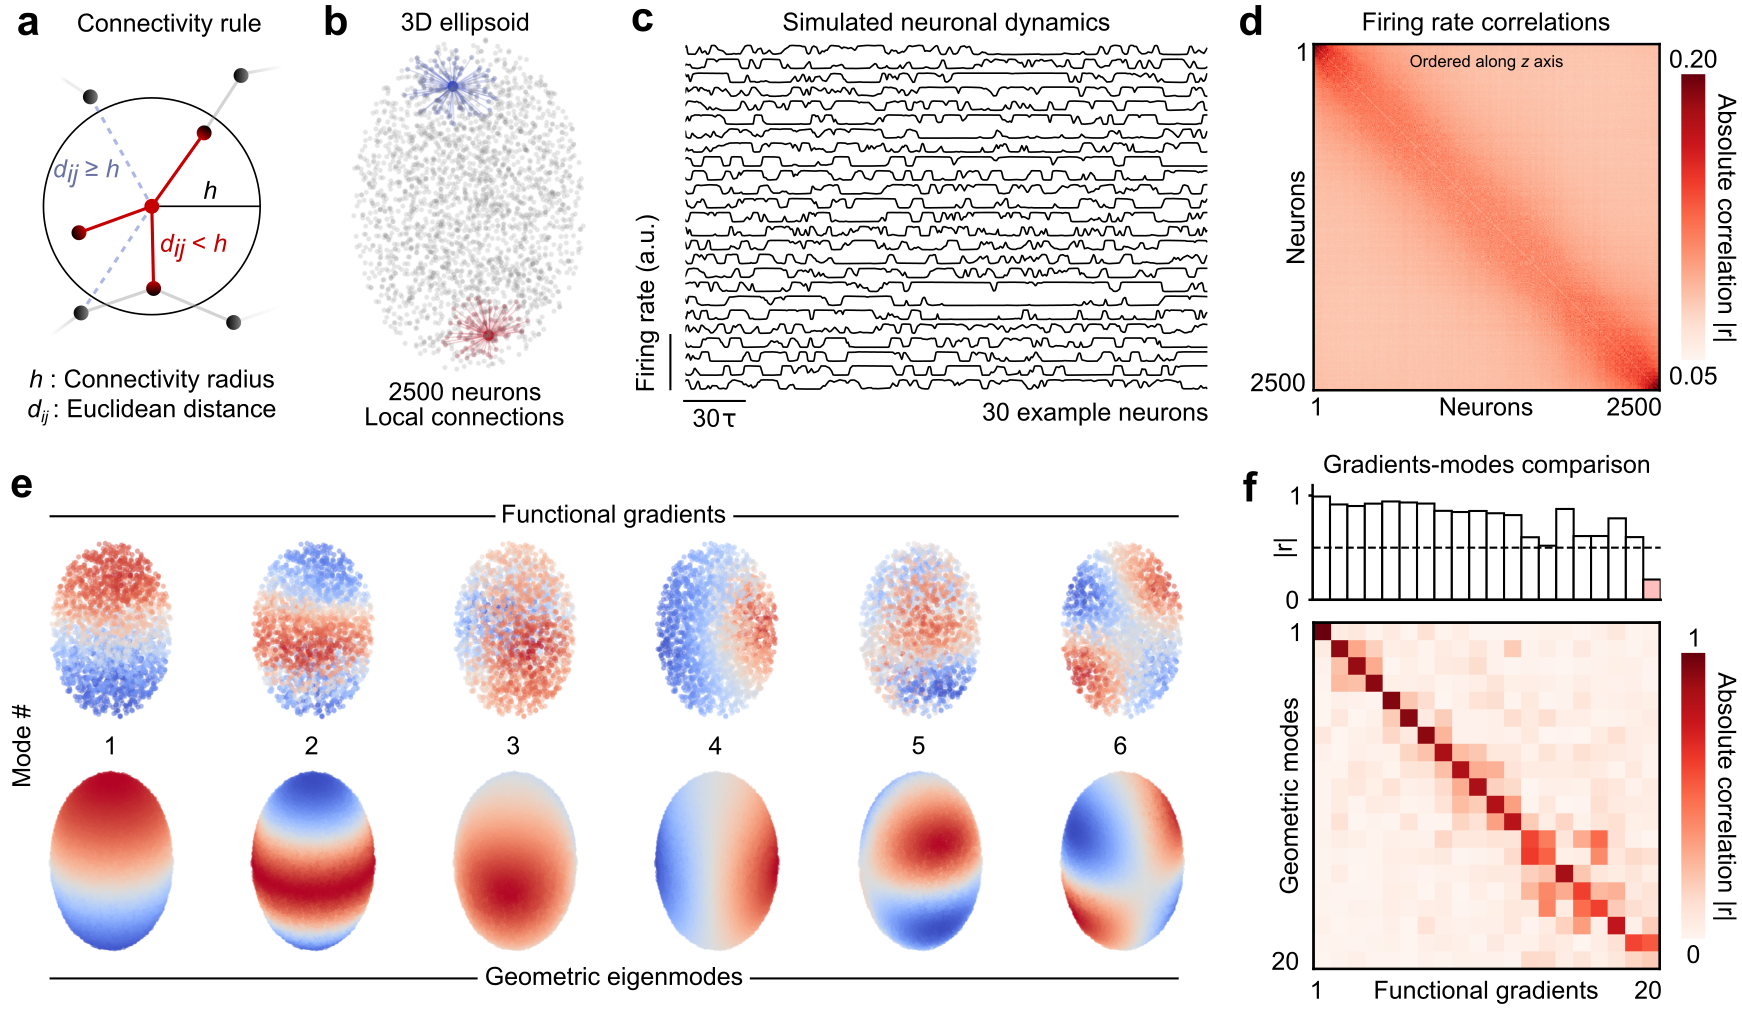
\includegraphics[width=0.95\textwidth]{Figures/figure1.png}
%    \caption{}
%    \label{fig1}
%\end{figure*}

\end{document}